\chapter[Metodologia]{Metodologia}

	Esta seção descreve todos os passos metodológicos utilizados para realização do trabalho, mostrando desde os equipamentos utilizados até como foram feitos os procedimentos de implementação, coleta e análise dos dados. 

\section{Levantamento Bibliográfico}

Uma vez escolhida a área de interesse e o tema, a primeira etapa do trabalho consistiu em um levantamento bibliográfico, a fim de avaliar a disponibilidade de material para fomentar o tema de trabalho de pesquisa e também analisar o que já foi desenvolvido na área. Feito isso, tomando-se como base o que já foi publicado e desenvolvido, foram definidas as possíveis contribuições, identificando (como foi dito na Seção 1 \ref{introduc}) a limitação de desempenho e o desenvolvimento para \textit{mobile} como áreas a serem exploradas.  

\section{Equipamentos Utilizados}

O celular utilizado foi o \textit{Nexus} 4, o qual é o quarto  \textit{smartphone} da  \textit{Google}, projetado e fabricado pela \textit{LG Electronics}.  Ele possui o processador \textit{Snapdragon S4 Pro} de 1,512 GHz \textit{quad-core}, GPU ( \textit{Graphics processing unit}) \textit{Adreno} 320 e 2 GB de memória RAM. O computador utilizado foi o da linha \textit{Alienware} M14x fabricado pela \textit{Dell}, no qual possui processador \textit{Intel Core} i7 de 2,3 GHz, GPU \textit{NVIDIA GeForce} GTX de 2 GB e 8 GB de memória RAM. 

\section{Configuração do Ambiente}
\label{configamb}	

	Em seguida, foram feitas as configurações dos ambientes de trabalho, em que  para desenvolver na plataforma \textit{Android} foi necessário instalar o \textit{Android SDK}, \textit{Android NDK} (para utilizar linguagem de código nativo C) e o \textit{plugin} ADT, uma vez que seria utilizada a IDE \textit{Eclipse}. A biblioteca gráfica para sistemas embarcados \textit{OpenGL ES} já é oferecida pela plataforma \textit{Android}. 

	Para poder realizar a coleta de métricas, foi utilizada a ferramenta \textit{Adreno Profiler}, pois o celular utilizado possui a GPU \textit{Adreno}. A \textit{Adreno Profiler} é uma ferramenta que foca na otimização gráfica para celulares que possuem GPU Adreno (fabricada pela empresa \textit{Qualcomm}). De acordo com  \cite{adp}, a ferramenta provê suporte para \textit{Android} e \textit{Windows RT} (variação do sistema operacional \textit{Windows} 8  e projetada para \textit{devices} móveis), permitindo a otimização, análise por quadros e visualização de desempenho em tempo real. No dispositivo \textit{Nexus 4} ela só é suportada com o \textit{Android} até a versão 4.3 (não suporta o \textit{KitKat}). 

	Como pode ser visto na Figura \ref{adrenoProfiler}, a ferramenta possui um módulo de análise dos \textit{vertex} e \textit{fragment} \textit{shaders}, sendo possível editá-los e analisar os resultados de compilação em tempo real, além dela também gerar estatísticas.  

	\begin{figure}[h]
	\centering
		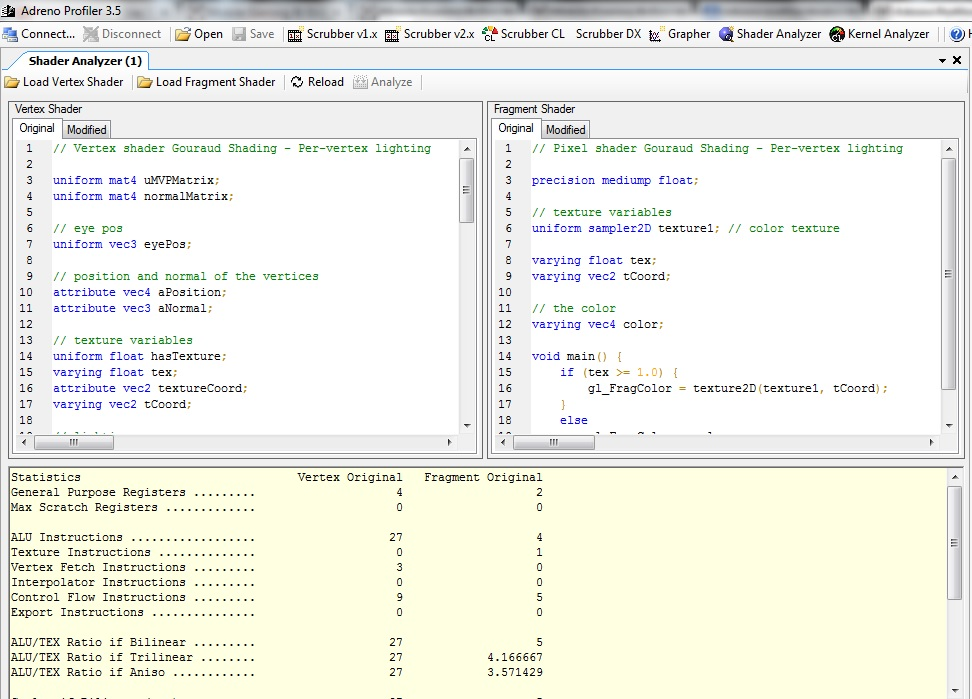
\includegraphics[keepaspectratio=true,scale=0.4]{figuras/shader_analyzer.jpg}
	\caption{Ferramenta \textit{Adreno Profiler}: analisador de \textit{shaders}}
	\label{adrenoProfiler}
	\end{figure}

	O módulo gráfico permite analisar algumas métricas, como as relacionadas ao \textit{vertex} e \textit{fragment shaders}, em que como é mostrado na Figura \ref{graph} um gráfico é plotado em tempo de execução. Além disso, ela também exporta os resultados no formato CSV (\textit{Comma-Separated Values}), que consiste em um arquivo de texto que armazena valores tabelados separados por um delimitador (vírgula ou quebra de linha). O último módulo é o chamado \textit{Scrubber}, que provê informações detalhadas quanto ao rastreamento de uma chamada de função. 

	\begin{figure}[h]
	\centering
		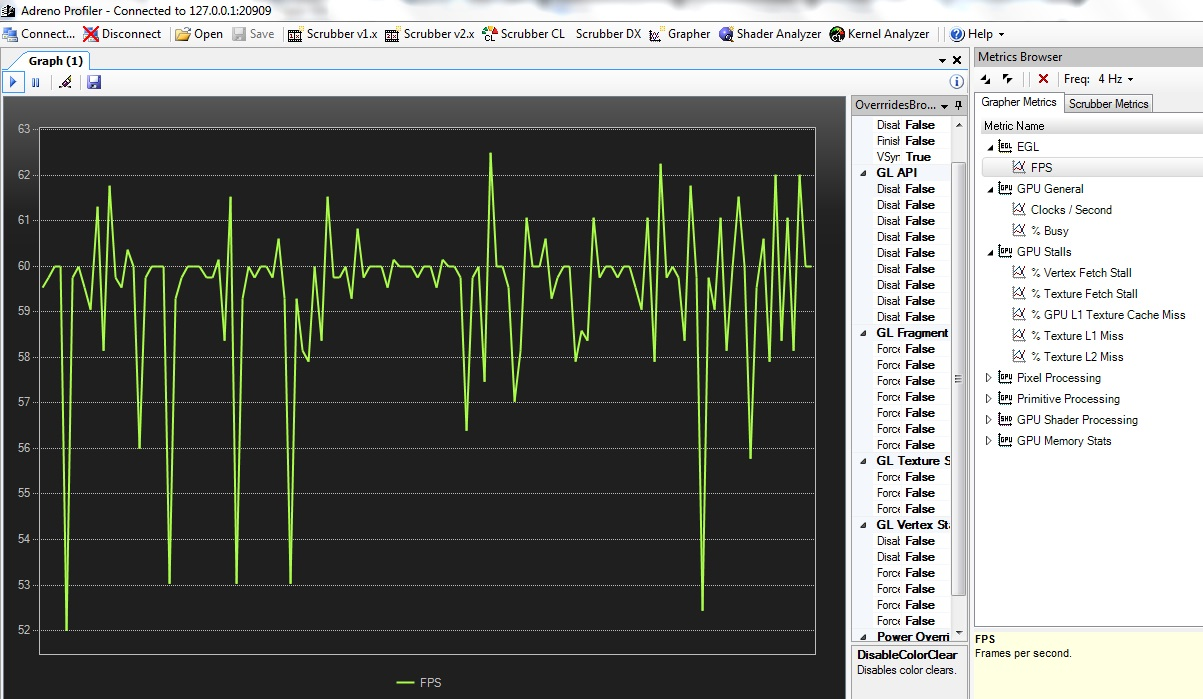
\includegraphics[keepaspectratio=true,scale=0.35]{figuras/graph.jpg}
	\caption{Ferramenta \textit{Adreno Profiler}: visualização de métrica quadros por segundo}
	\label{graph}
	\end{figure}

	Para a automatização da plotagem dos gráficos e aplicação do método dos mínimos quadrados (descrito na seção \ref{metminqua}) utilizou-se a linguagem de programação Python \footnote{http://www.python.org.br/} versão 2.3.7, juntamente com os pacotes  \textit{matplotlib} \footnote{http://www.matplotlib.org/} e  \textit{numpy} \footnote{http://www.numpy.org/}. 

	O controle de versionamento do código foi feito por meio do sistema de controle de versão Git \footnote{http://git-scm.com/} utilizando o \textit{forge} GitHub \footnote{https://github.com/}. Foram criados repositórios públicos tanto para a implementação em \textit{Android} \footnote{https://github.com/campeloal/monografia\_opengles} quanto para a automatização da análise da complexidade algorítmica \footnote{https://github.com/campeloal/monografia\_algorithmComplexity/}. 

\section{Implementação Plataforma \textit{Android}} 
\label{imp}

	 A fim de tornar possível a realização da análise da complexidade algorítmica experimentalmente, primeiramente focou-se na implementação dos \textit{shaders} para plataforma \textit{Android} utilizando a biblioteca \textit{OpenGL ES}. Foi utilizado  o paradigma de orientação a objetos, em que o diagrama de classes (Figura \ref{class_diagram}) mostra como ele está estruturado. Ele mostra um conjunto de classes e seus relacionamentos, sendo o diagrama central da modelagem orientada a objetos. 

	\begin{figure}[h]
	\centering
		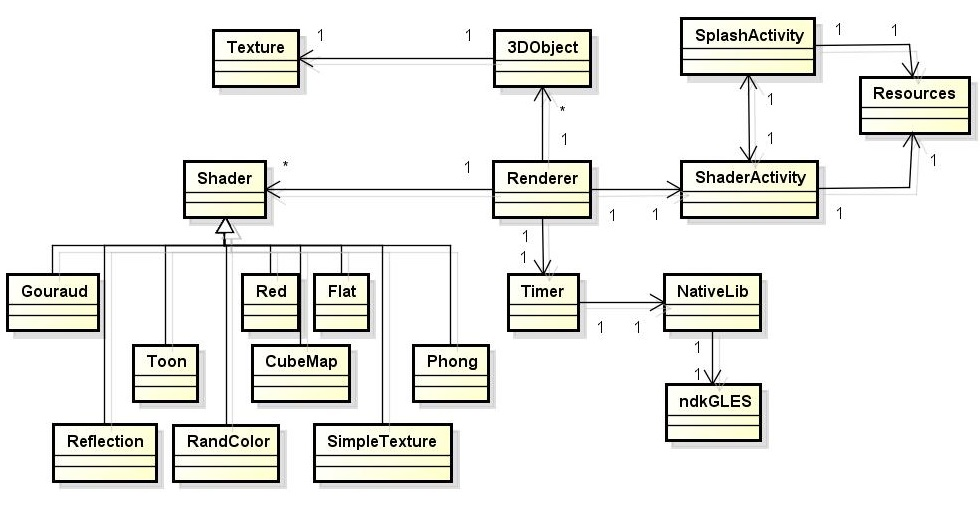
\includegraphics[keepaspectratio=true,scale=0.6]{figuras/class_diagram.jpg}
	\caption{Diagrama de Classe da Implementação em \textit{Android}}
	\label{class_diagram}
	\end{figure}

\subsection{Classes \textit{Shader Activity} e \textit{Splash Activity}}

	\begin{figure}[h]
	\centering
		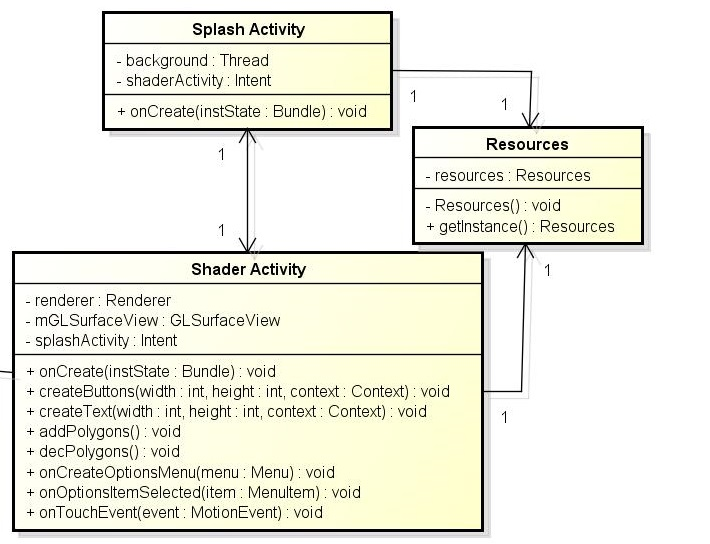
\includegraphics[keepaspectratio=true,scale=0.6]{figuras/shader_splash.jpg}
	\caption{Detalhamento das classes \textit{Shader Activity}, \textit{Splash Activity} e \textit{Resources}}
	\label{shader_splash}
	\end{figure}

	De acordo com \ref{androidsdkmanager}, a plataforma \textit{Android} utiliza o termo \textit{Activity} para descrever a tela de \textit{front-end} da aplicação que interage com o usuário. Ela possui elementos de \textit{design} como texto, botões, gráficos, entre outros. No contexto deste trabalho, há duas classes \textit{Activity}, a \textit{Shader} e a \textit{Splash}. 

	A \textit{Splash Activity} (Figura  \ref{splash_act}) é responsável pela visualização da tela de \textit{loading} enquanto carrega os recursos necessários para o programa (como a leitura dos modelos tridimensionais em formato obj e das imagens usadas para texturização) por meio do uso de \textit{thread}. Estes recursos são setados por meio da classe chamada \textit{Resources}, que utiliza o padrão de projeto chamado \textit{Singleton}, que garante a existencia de apenas uma instância da classe, que será acessada posteriormente.

	\begin{figure}[h]
	\centering
		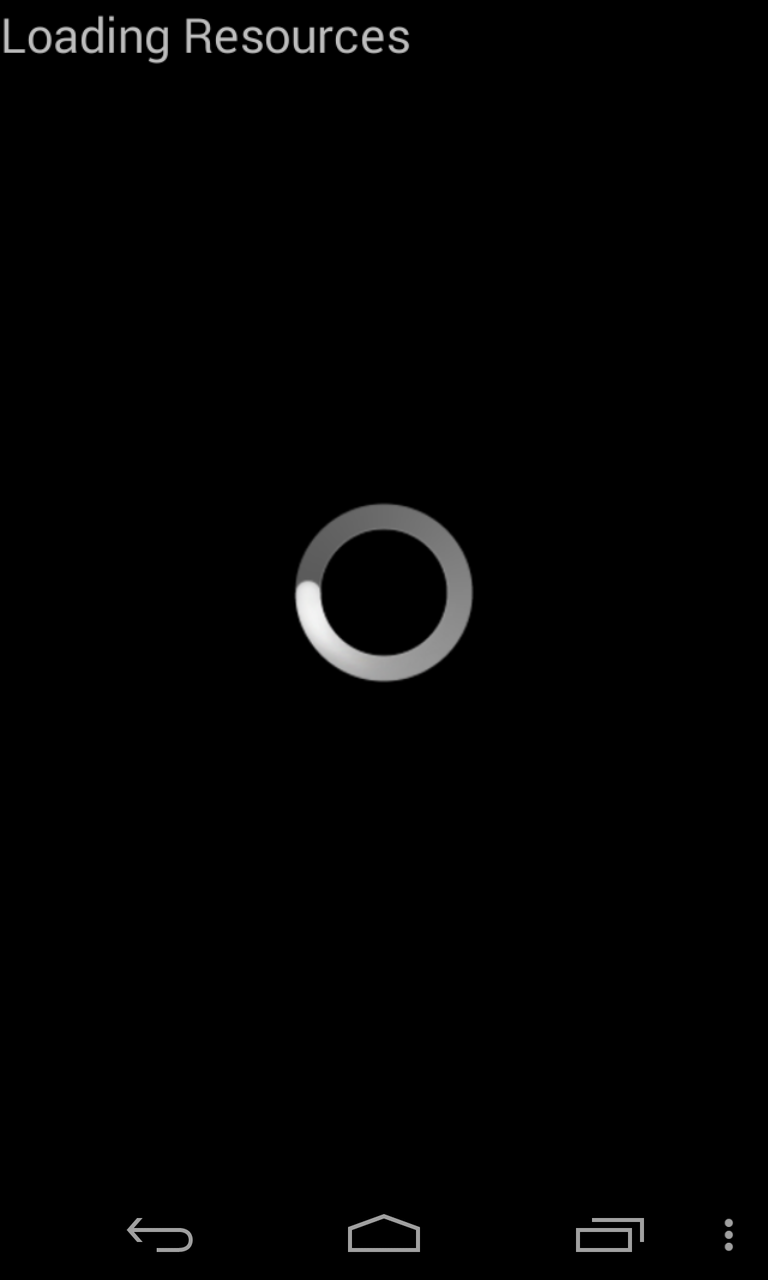
\includegraphics[keepaspectratio=true,scale=0.2]{figuras/splash_act.png}
	\caption{Tela da \textit{Splash Activity}}
	\label{splash_act}
	\end{figure}

	A \textit{Shader Activity} (Figura  \ref{shader_act}) é responsável pela  instanciação da classe \textit{Renderer}, que renderiza os gráficos tridimensionais utilizando a biblioteca \textit{OpenGL ES}. Além disso, ela controla os eventos de \textit{touch}, que permitem escalar e mover o objeto, além de disponibilizar os menus que trocam de \textit{shaders}, os botões que aumentam, diminuem o número de polígonos, a informação do tempo de renderização e a de quantidade de polígonos. Aumenta-se o número de polígonos por meio da troca de objetos que possuem arquivos obj diferentes, que já foram carregados pela \textit{Splash Activity}. 

	\begin{figure}[h]
	\centering
		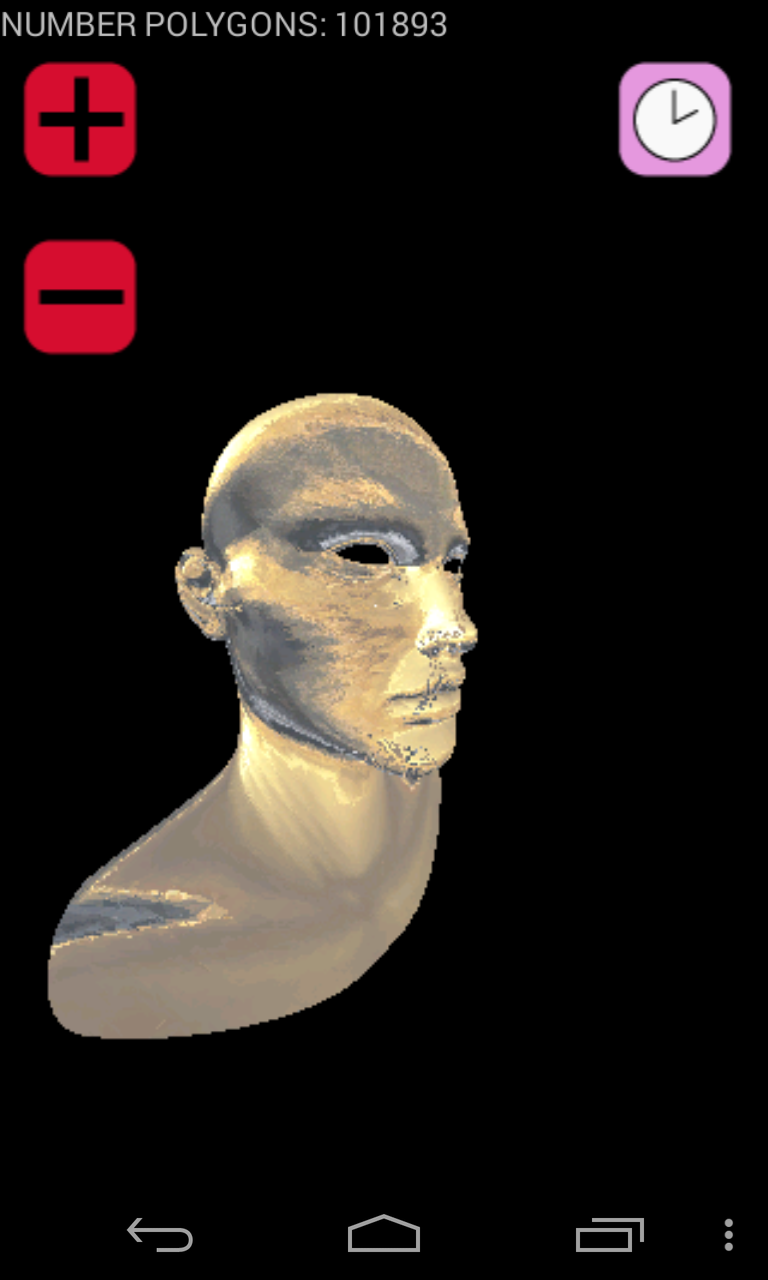
\includegraphics[keepaspectratio=true,scale=0.2]{figuras/shader_act.png}
	\caption{Tela da \textit{Shader Activity}}
	\label{shader_act}
	\end{figure}

	Devido à limitação de memória do dispositivo móvel e os vários objetos com diferentes números de polígonos, não é possível carregar todos de uma só vez. Assim, foi necessário dividir esta quantidade objetos por vez, em que quando chega-se ao último objeto (tanto adicionando, quanto decrementando), volta-se novamente para a \textit{Splash Activity}, a fim de carregar os novos objetos e ir novamente para a \textit{Shader Activity}, a fim de renderizá-los.

\subsection{ Classes \textit{3DObject} e \textit{Texture}}   

	\begin{figure}[h]
	\centering
		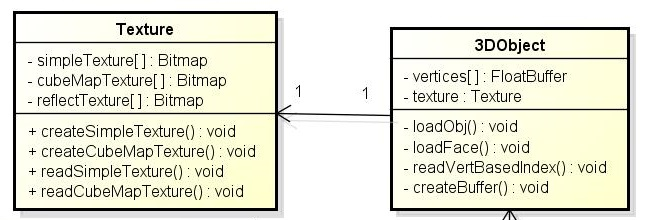
\includegraphics[keepaspectratio=true,scale=0.6]{figuras/object_texture.jpg}
	\caption{Detalhamento das classes \textit{3DObject} e \textit{Texture}}
	\label{object_texture}
	\end{figure}

	A classe \textit{3DObject}, mostrada na Figura \ref{object_texture}, é responsável por ler e interpretar os arquivos  \textit{obj}  (descrito na Seção \ref{formatobj}). . Estes arquivos foram criados e exportados utilizando a ferramenta de modelagem tridimensional \textit{open-source} chamada Blender \footnote{http://www.blender.org/} como pode ser visto na Figura \ref{blender}. Ela também permite modificar o número de polígonos a partir de um modelo tridimensional, por meio de modificadores chamados \textit{Decimate} e \textit{Subdivision Surface} (usados para diminuir e aumentar a contagem poligonal, respectivamente).  Assim, foi possível variar a contagem poligonal a partir de diferentes arquivos \textit{obj}.

	\begin{figure}[h]
	\centering
		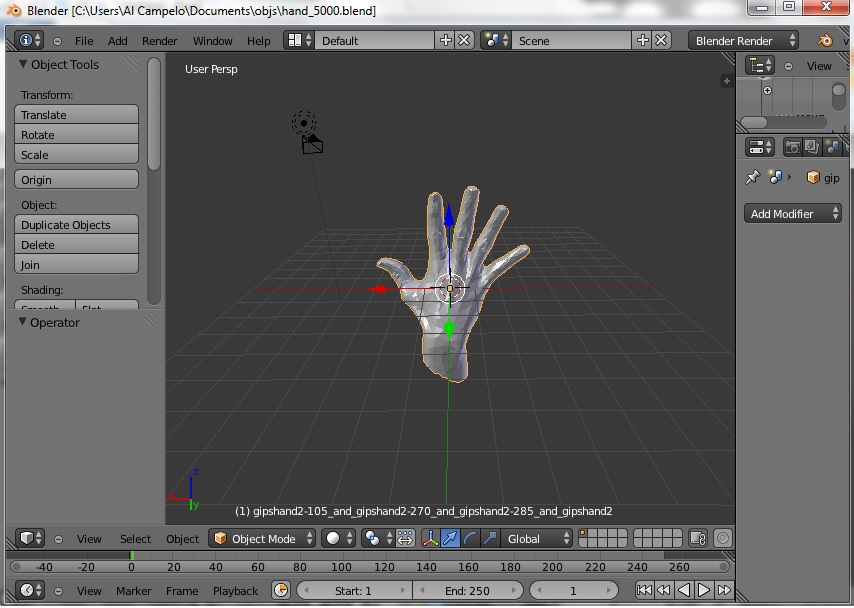
\includegraphics[keepaspectratio=true,scale=0.7]{figuras/blender.jpg}
	\caption{Ferramenta de modelagem tridimensional}
	\label{blender}
	\end{figure}

	Após a leitura e interpretação do arquivo \textit{obj} é gerado um \textit{buffer} que armazena os vértices de posição, normal e textura na ordem em que eles serão renderizados. Nele cada coordenada relacionada a um vértice (posição, normal e textura) é armazenada alternadamente, como mostra a Figura \ref{buffer}.

	\begin{figure}[h]
	\centering
		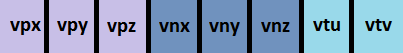
\includegraphics[keepaspectratio=true,scale=1.0]{figuras/buffer.png}
	\caption{Ordem das coordenadas de posição, normal e textura para um vértice}
	\label{buffer}
	\end{figure}

	A classe \textit{Texture} gera as texturas utilizadas pelos \textit{shaders} \textit{SimpleTexture}, \textit{CubeMap} e \textit{Reflection} baseando-se em imagens. As imagens são criadas para cada modelo tridimensional, utilizando a técnica de \textit{UV Mapping}, na qual mapeiam-se as coordenadas de textura para uma imagem ( Figura \ref{uvmap}). Como a orientação do eixo de coordenas y da ferramenta \textit{Blender} é diferente da \textit{OpenG ES}, é necessário virar a imagem neste eixo para correto mapeamento.

	Para gerar uma textura simples, primeiramente gera-se um objeto de textura \texttt{glGenTextures}, depois vincula-se a a textura a este objeto utilizando a função \texttt{glBindTexture} e carrega-se a imagem por meio da função \texttt{texImage2D}.  Para as texturas do \textit{CubeMap} e \textit{Reflection}, faz-se a mesma coisa, exceto que a função \textit{texImage2D} é feita seis vezes, em que cada textura representa uma face de um cubo. 

	\begin{figure}[h]
	\centering
		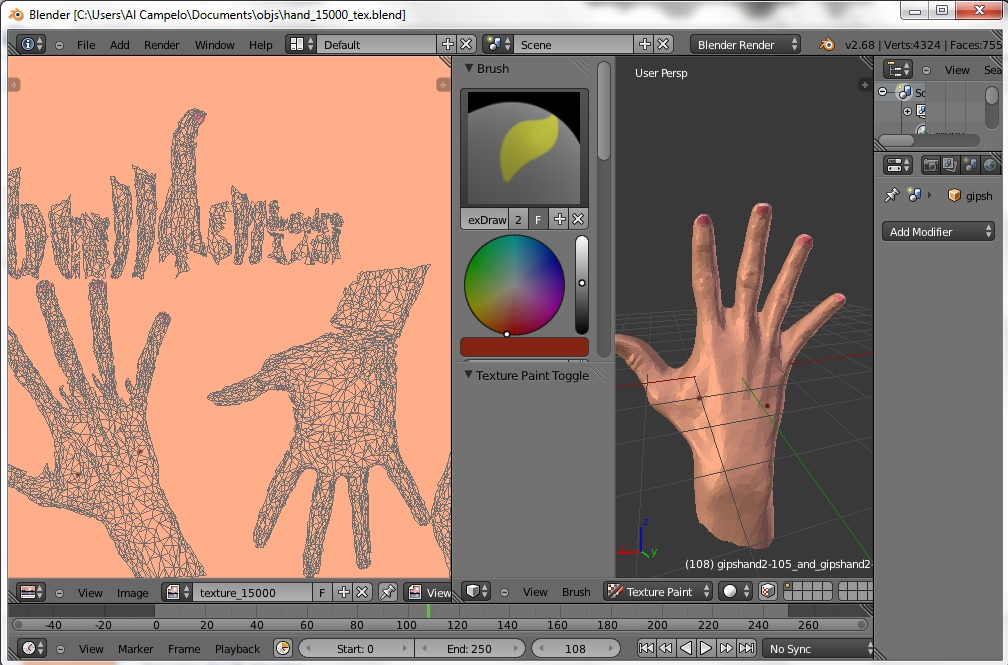
\includegraphics[keepaspectratio=true,scale=0.6]{figuras/uvmap.jpg}
	\caption{Técnica de mapeamento de textura utilizada para cada modelo 3D}
	\label{uvmap}
	\end{figure}

	Na Figura  \ref{texture_uvmap} é mostrada a imagem resultante da técnica de mapeamento realizada.

	\begin{figure}[h]
	\centering
		
\includegraphics[keepaspectratio=true,scale=0.2]{figuras/texture_uvmap.jpg}
	\caption{Textura gerada a partir da técnica de mapeamento}
	\label{texture_uvmap}
	\end{figure}

\subsection{Classes \textit{Timer} e \textit{NativeLib}}      

	\begin{figure}[h]
	\centering
		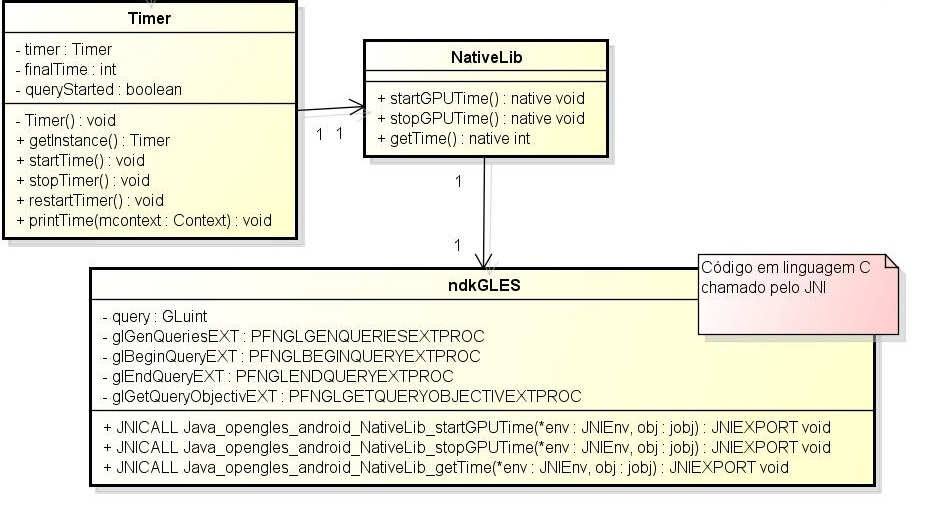
\includegraphics[keepaspectratio=true,scale=0.6]{figuras/timer_nativelib.jpg}
	\caption{Detalhamento das classes \textit{Timer} e \textit{NativeLib}}
	\label{timer_nativelib}
	\end{figure}

	A Figura \ref{timer_nativelib} detalha a classe \textit{Timer}, que realiza a média de dez medições do tempo (em nanosegundos) para cada objeto tridimensional, utilizando um \textit{shader} específico. Cada medição é feita utilizando a linguagem C e a extensão de \textit{OpenGL ES} chamada GL\_EXT\_disjoint\_timer\_query citada na Seção \ref{gpu}.  A integração entre o codigo em linguagem C e o código em Java é feita por meio da classe \textit{NativeLib}.

\subsection{Classe \textit{Renderer}}    

	\begin{figure}[h]
	\centering
		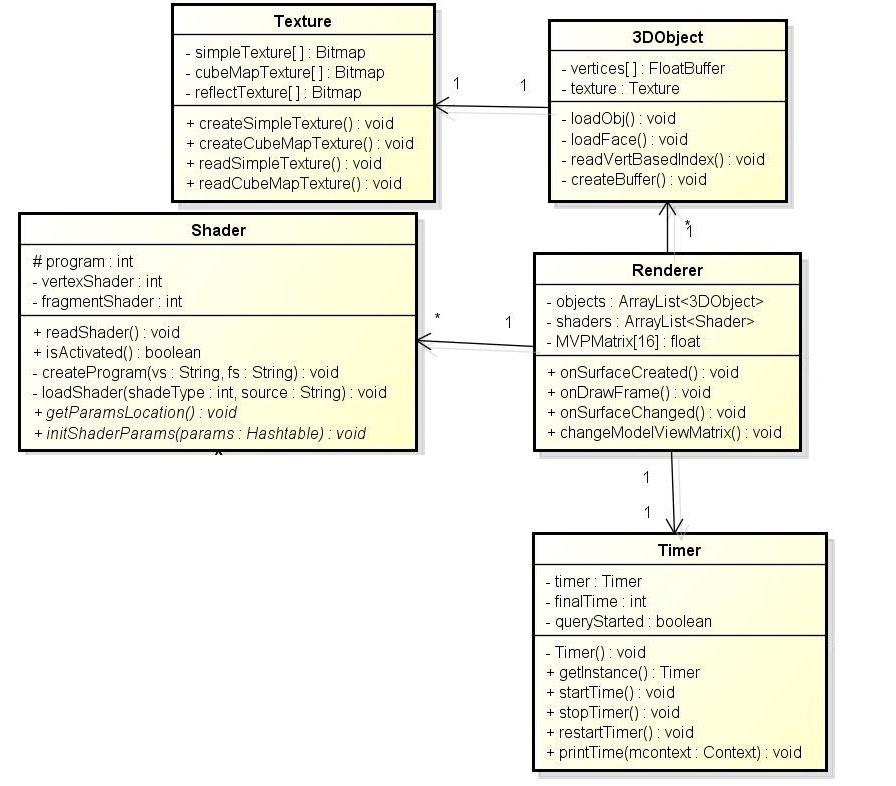
\includegraphics[keepaspectratio=true,scale=0.6]{figuras/renderer.jpg}
	\caption{Detalhamento da classe \textit{Renderer}}
	\label{renderer}
	\end{figure}

	A classe \textit{Renderer} (Figura \ref{renderer}) funciona como uma controladora, sendo o ponto principal  das chamadas provenientes da \textit{view} (\textit{ShaderActivity}) para a camada mais abaixo (\textit{3DObject}, \textit{Shader} e \textit{Timer}). Ela que implementa as funções da biblioteca \textit{OpenGL ES} \texttt{onSurfaceCreated},  \texttt{onDrawFrame} e \texttt{onSurfaceChanged}. A primeira função é chamada apenas uma vez quando a \textit{view} da \textit{OpenGL ES} é instanciada, em que faz-se todas as configurações nesta função, como por exemplo, criação de texturas. A segunda função é chamada em \textit{loop}, em que faz-se a renderização por meio da função \texttt{glDrawArrays}. 

\subsection{Classe \textit{Shader}}      

	\begin{figure}[h]
	\centering
		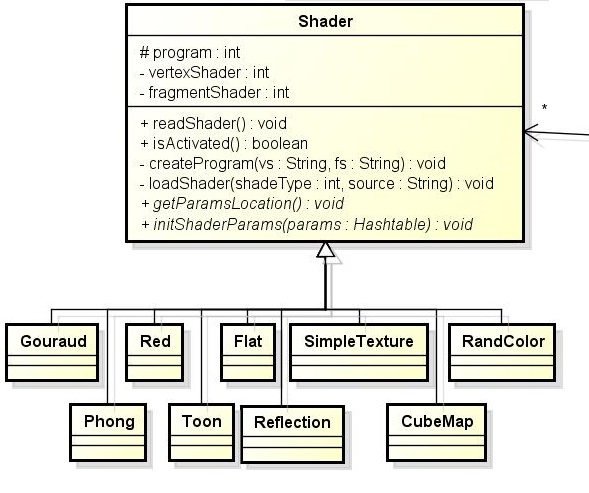
\includegraphics[keepaspectratio=true,scale=0.6]{figuras/shaders_diag.jpg}
	\caption{Detalhamento da classe \textit{Shader}}
	\label{shaders_diag}
	\end{figure}

	A classe \textit{Shader} (Figura \ref{shaders_diag}) é responsável por ler, fazer o \textit{attach} e o \textit{link} do \textit{ vertex} e do \textit{fragment shaders}. Além disso, ela possui os métodos abstratos \texttt{getParamsLocation} e \texttt{initShaderParams(Hastable params)}. Assim, todos os \textit{shaders} que herdam desta classe, são obrigados a implementar estes métodos. O primeiro método faz o armazenamento da localização de cada variável especificada dentro do \textit{shader}, já o segundo método inicializa estas variáveis por meio de um \textit{hash} que é passado como um parâmetro pela classe \textit{Renderer}. Assim, todos os \textit{shaders} implementados herdam da classe \textit{Shader} e implementam seus métodos abstratos. Estes \textit{shaders} podem ser vistos na Figura \ref{shaders_impl}.  

	\begin{figure}[h]
	\centering
		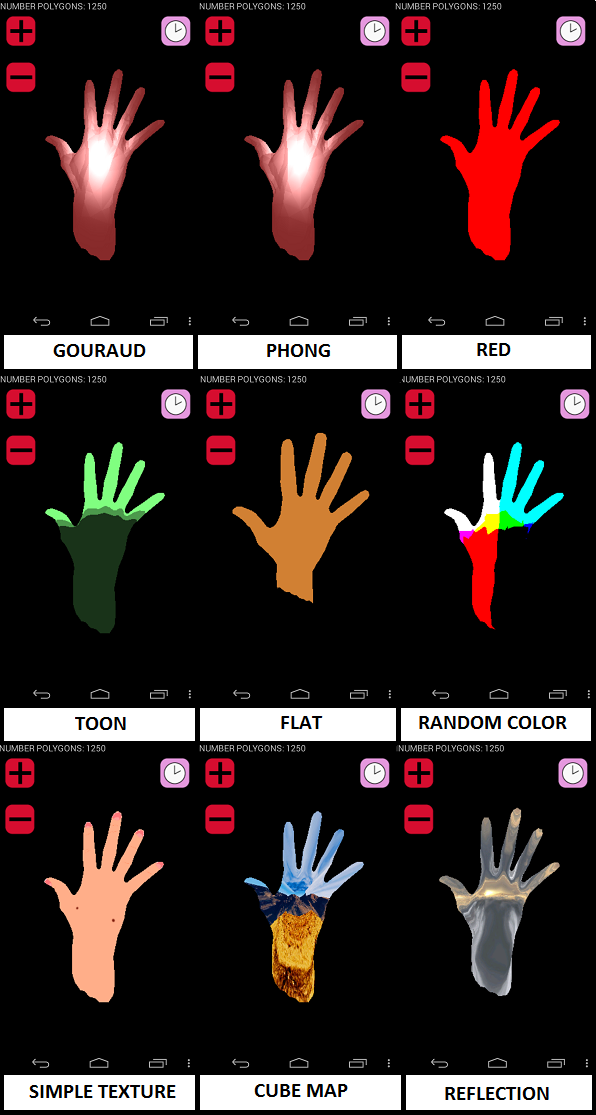
\includegraphics[keepaspectratio=true,scale=0.7]{figuras/shaders_impl.png}
	\caption{\textit{Shaders} Implementados}
	\label{shaders_impl}
	\end{figure}

	A seguir, alguns dos \textit{shaders} implementados serão explicados:

\subsubsection{\textit{Phong Shader}}

	O \textit{vertex} e \textit{fragment shaders} do \textit{phong shading} implementam a técnica descrita na Seção \ref{flatgouphon}, em que primeiramente interpolam-se os valores das normais das primitivas e então computam-se os cálculos de luz para cada fragmento, utilizando as normais interpoladas. O Código \ref{codphongvs} e o Código \ref{codphongfs} mostram as definições do \textit{vertex} e \textit{fragment shaders}, respectivamente, em que para isso é necessário definir as propriedades do material pelo programa.  

	\lstinputlisting[language=C, label = {codphongvs}, caption = {\textit{Phong Shader}:  \textit{vertex shader}}]{codigos/phong_vs.txt}

	\lstinputlisting[language=C, caption =  {\textit{Phong Shader}:  \textit{fragment shader}}, label = {codphongfs}  ]{codigos/phong_ps.txt}
	
\subsubsection{\textit{Red Shader}}
	
	O \textit{shader} que define a cor para vermelha é muito simples,  seu \textit{vertex shader} apenas estabelece que a posição do vértice  se dá pelo pela multiplicação da coordenada ( variável \texttt{aPosition} ) com a matriz de projeção, visualização e modelagem como é mostrada no Código \ref{codredvs}. 
	
	\lstinputlisting[language=C, caption = {\textit{Red Shader}:  \textit{vertex shader}}, label = {codredvs}]{codigos/red_vs.txt}

	Já o seu \textit{fragment shader} (Código \ref{codredfs}) estabele que todo fragmento possui a cor vermelha, por meio da palavra restrita \texttt{gl\_FragColor}.
	
	\lstinputlisting[language=C, caption = {\textit{Red Shader}:  \textit{fragment shader}}, label = {codredfs}]{codigos/red_ps.txt}

\subsubsection{\textit{Toon Shader}}

	O  \textit{toon shader} calcula a intensidade da luz por vértice para escolher uma das cores pré-definidas, como é explicado na Seção ADICIONAR SEÇÃO. O Código  \ref{codtoonvs} mostra o cálculo da intensidade da luz por vértice, pegando primeiro a direção da luz (definida como uma variável \texttt{uniform} passada pelo programa) para depois fazer o produto escalar entre ela e a normal (cálculo da intensidade da luz).  

	\lstinputlisting[language=C,label = {codtoonvs}, caption = {\textit{Toon Shader}:  \textit{vertex shader}} ]{codigos/toon_vs.txt}

	A variável \textit{intensity} do tipo \textit{varying} é passada do \textit{vertex shader} para o \textit{fragment shader}, a fim de determinar qual das três cores será escolhida (Código \ref{codtoonfs}). 
  
 	\lstinputlisting[language=C, caption = {\textit{Toon Shader}:  \textit{fragment shader}}, label = {codtoonfs} ]{codigos/toon_ps.txt}

\subsubsection{\textit{Simple Texture Shader}}

	O \textit{vertex shader} do \textit{simple texture shading} primeiramente armazena as coordenadas de textura numa variável do tipo \textit{varying} (Código \ref{codtexvs}), e as repassa para o \textit{fragment shader}, além de também definir a posição.  

	\lstinputlisting[language=C, caption =  {\textit{Simple Texture Shader}:  \textit{vertex shader}}, label = {codtexvs} ]{codigos/simple_tex_vs.txt}

	No Código \ref{codtexfs}, o \textit{fragment shader} por sua vez, utiliza a textura passada pelo programa e aplica a coordenada de textura, repassada pelo \textit{vertex shader}, no fragmento por meio da função  \texttt{texture2D}.

	\lstinputlisting[language=C, caption =  {\textit{Simple Texture Shader}:  \textit{fragment shader}}, label = {codtexfs} ]{codigos/simple_tex_ps.txt}

\subsubsection{\textit{CubeMap Shader}}	

	 O \textit{CubeMap Shader} implementa a técnica descrita na Seção ADICIONAR SEÇÃO. O seu  \textit{vertex shader} é simples e só define a posição do vértice (Código \ref{codcubemapvs}). 

	\lstinputlisting[language=C, caption =  {\textit{CubeMap Shader}:  \textit{vertex shader}}, label = {codcubemapvs} ]{codigos/cubemap_vs.txt}

	O  \textit{fragment shader} (Código \ref{codcubemapps}), por sua vez, utiliza a função \texttt{textureCube} utiliza a normal para fazer o mapeamento da textura. 

	\lstinputlisting[language=C, caption =  {\textit{CubeMap Shader}:  \textit{fragment shader}}, label = {codcubemapps} ]{codigos/cubemap_ps.txt}
	
\subsubsection{\textit{Reflection Shader}}

	O \textit{vertex shader} do \textit{shader} de reflexão é responsável por indicar que a posição do vértice se dá pela multiplicação da coordenada obtida pela variável \texttt{vec4 aPosition} com a matriz de projeção, visualização e modelagem, como é mostrado no Código \ref{codreflvs}. Além disso, ele declara dois vetores do tipo \textit{varying} (para passar ao \textit{fragment shader}) que estão relacionados com o vetor de direção da câmera e a normal. 

	\lstinputlisting[language=C, caption = {\textit{Reflection Shader}:  \textit{vertex shader}}, label = {codreflvs}]{codigos/reflection_vs.txt}

	No \textit{fragment shader}, a normal e o vetor de direção da câmera são utilizados para encontrar o vetor da direção da reflexão através da utilização da função \texttt{reflect}. Para corrigir a direção da normal, ela é multiplicada pela transposta da inversa da matriz de projeção, modelagem e visualização, como foi explicado na seção ADICIONAR LINK PARA SEÇÃO. O vetor da direção da reflexão é utilizado na função \textit{textureCube} (Código \ref{codreflfs}), em que determina-se a cor do fragmento, baseando-se nesta direção e em uma imagem. 

	\lstinputlisting[language=C, caption = {\textit{Reflection Shader}:  \textit{fragment shader}}, label = {codreflfs}]{codigos/reflection_ps.txt}

\section{Análise da Complexidade Algorítmica Experimentalmente}

	A análise da complexidade algorítmica, experimentalmente, foi feita coletando-se diversas medições para cada modelo tridimensional (com diferentes quantidades de polígonos), e em seguida, os gráficos foram plotados e ajustados à uma curva.  

\subsection{Medição do Tempo de Renderização Realizada pela GPU}
\label{gpu}

	A fim de realizar a análise de complexidade algorítmica, primeiro buscou-se coletar uma métrica relacionada ao tempo de renderização dos \textit{shaders}. E por meio de pesquisa e consulta na documentação da \textit{OpenGL ES} conseguiu-se encontrar uma extensão desta biblioteca gráfica que permite contabilizar o tempo, em nanosegundos, necessário para realizar chamadas de \textit{OpenGL ES} especificadas. Esta extensão se chama GL\_EXT\_disjoint\_timer\_query \footnote{http://www.khronos.org/registry/gles/} e só está disponível para o dispositivo \textit{Nexus 4} a partir da versão de Android 4.4 ( \textit{KitKat}).

	Para utilizar esta extensão foi necessário instalar e configurar o NDK ( \textit{Native Development Kit}) e alterar o \textit{header} da versão da \textit{OpenGL ES} utilizada, adicionando as linhas de código relacionadas à extensão almejada. Assim, foi possível utilizar as novas funções desta extensão pegando os seus endereços por meio do comando eglGetProcAddress ( disponível por meio da API EGL que faz o interfaceamento entre a \textit{OpenGL ES} e o sistema operacional). A integração entre o codigo em linguagem C e o código em Java é feita por meio do JNI (\textit{Java Native Interface}).

	Feita a configuração e implementação da coleta de tempo para execução da função \textit{glDrawArrays} (responsável pela renderização), foram plotados os gráficos - para cada \textit{shader} - do tempo em nanosegundos \textit{versus} a quantidade de polígonos. Porém, após feita as plotagens para todos os \textit{shaders}, foi possível perceber que as formas de todas as funções se assemelhavam a uma exponencial (como é visto na Figura  \ref{ndk_exp} referente ao \textit{phong shader}). É possível ver esta semelhança trocando-se a escala do grafico natural para logarítmica (apenas no eixo y), pois uma exponencial nesta escala vira uma reta (como demonstrado na Seção \ref{metminqua} e na  Figura  \ref{ndk_reta}). Então, chegou-se à conclusão que ao se coletar o tempo de realização da função \textit{glDrawArrays}, estava-se contabilizando todo o processo de renderização e não somente o de aplicação do \textit{vertex} e  \textit{fragment}  \textit{shaders}. Então, viu-se necessário a coleta de métricas específicas relacionadas ao \textit{vertex} e \textit{fragment} \textit{shaders}. 

	\begin{figure}[h]
	\centering
		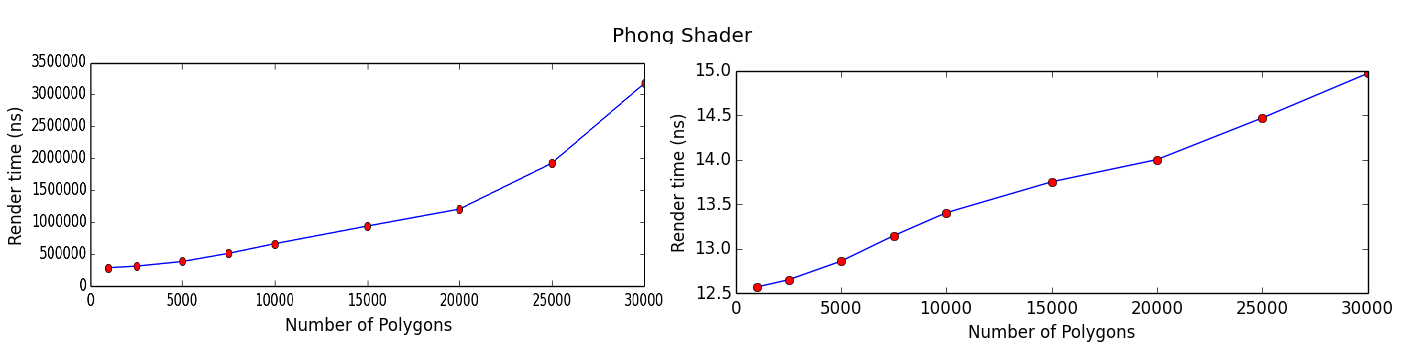
\includegraphics[keepaspectratio=true,scale=0.6]{figuras/ndk_exp.png}
	\caption{Gráfico em escala natural}
	\label{ndk_exp}
	\end{figure}

	\begin{figure}[h]
	\centering
		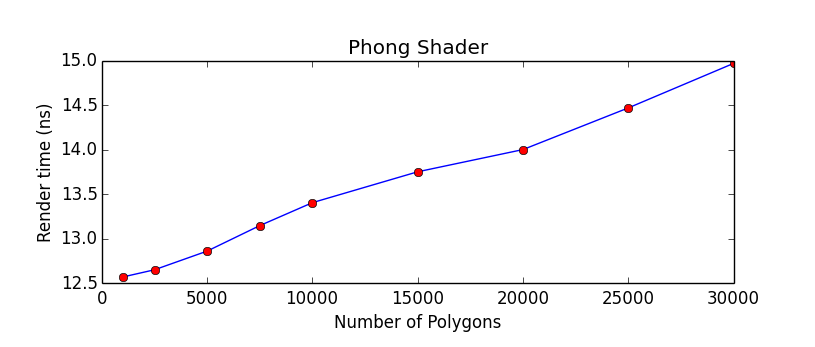
\includegraphics[keepaspectratio=true,scale=0.6]{figuras/ndk_reta.png}
	\caption{Gráfico em escala logarítmica}
	\label{ndk_reta}
	\end{figure}

\subsection{Medição do Número de Instruções por Segundo, Plotagem e Ajuste das Curvas}

	Para a coleta de medições relacionadas ao \textit{vertex} e \textit{fragment} \textit{shaders}, utilizou-se a ferramenta \textit{Adreno Profiler}. As métricas escolhidas foram a de número de instruções por segundo por vértice e número de instruções por segundo por fragmento e elas foram coletadas para cada número específico de polígonos, sendo exportadas no formato CSV. 	A fim de ajustar as curvas a uma função, e consequentemente analisar a complexidade algorítmica, utilizou-se o método dos mínimos quadrados (Seção Seção \ref{metminqua}) para uma função linear, quadrática, cúbica e exponencial, calculando-se os respectivos erros, e podendo assim, descobrir qual curva se aproxima mais. 

	 Para automatizar estas etapas descritas anteriormente, foi feito um programa em Python que lê os arquivos CSV, faz a média das medições, plotagens dos gráficos para o \textit{vertex} e \textit{fragment} \textit{shaders} e realiza os ajustes das curvas, calculando os erros associados e qual o menor entre eles. Ele é executado por linha de comando, em que passa-se como parâmetro o \textit{shader} desejado (Figura \ref{linhacomando}).

	\begin{figure}[h]
	\centering
		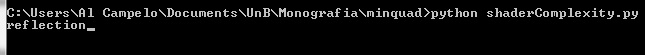
\includegraphics[keepaspectratio=true,scale=1.0]{figuras/linhacomando.jpg}
	\caption{Linha de comando para execução do programa}
	\label{linhacomando}
	\end{figure}


	O programa encontra-se estruturado de acordo com a Figura \ref{minquad_diag}, em que a classe \textit{ReadCSV} é responsável por ler os arquivos CSV e fazer a média das métricas tanto para o \textit{vertex shader} como para o \textit{fragment shader}. Já a classe \textit{PlotChart}, faz a plotagem do gráfico do número de instruções por segundo por vértice \textit{versus} o número de polígonos e do gráfico do número de instruções por segundo por fragmento \textit{versus} o número de polígonos. Além disso, ele também plota o gráfico original juntamente com o gráfico após a aplicação do método dos mínimos quadrados. Por fim, o módulo \textit{LeastSquares} realiza o ajuste dos mínimos quadrados para uma reta, uma exponencial e para polinômios de segundo e terceiro graus. Este módulo também calcula os erros associados a cada ajuste e indica qual o menor. 

	\begin{figure}[h]
	\centering
		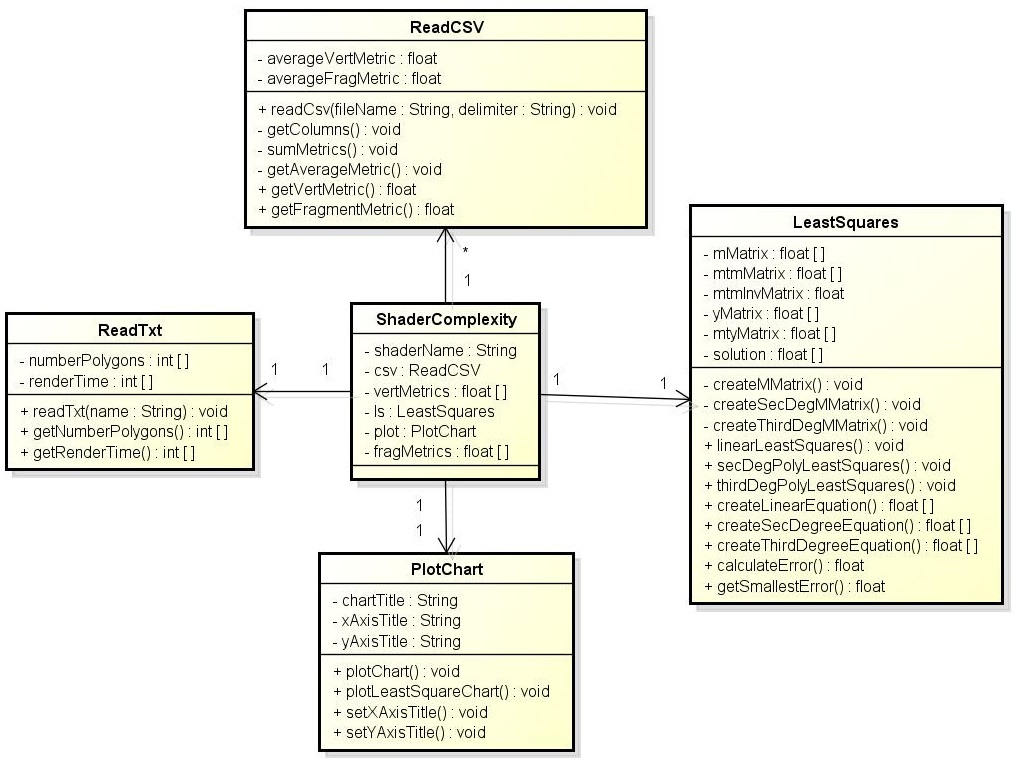
\includegraphics[keepaspectratio=true,scale=0.6]{figuras/minquad_diag.jpg}
	\caption{Diagrama de Classes do código de automatização}
	\label{minquad_diag}
	\end{figure}

